\documentclass{article}
\usepackage[utf8]{inputenc}      % Codificación de entrada UTF-8
\usepackage[T1]{fontenc}         % Codificación de salida T1
\usepackage[official]{eurosym}   % Símbolo de euro
\usepackage{siunitx}             % Paquete para unidades métricas
\usepackage{textcomp}            % Tipografías compañeras
\usepackage{lmodern}             % Tipografía Latin Modern
\usepackage{moreverb}            % Para escribir código
\usepackage{tfrupee}
\usepackage{fontawesome5}
\usepackage{parskip}
\usepackage{hyperref}
\usepackage{tasks}
\usepackage{exsheets}
\usepackage{enumitem}
\usepackage{lastpage}
\usepackage{booktabs}
\usepackage{graphicx}
\usepackage{apalike}
\usepackage{relsize}
\usepackage{listings}
\usepackage{amsmath}
\usepackage{amssymb}

% Code listing style
\lstset{
    language=Python,
    basicstyle=\ttfamily\footnotesize,
    keywordstyle=\color{blue},
    commentstyle=\color{gray},
    stringstyle=\color{green!60!black},
    numbers=left,
    numberstyle=\tiny\color{gray},
    numbersep=5pt,
    breaklines=true,
    showstringspaces=false,
    frame=single,
    backgroundcolor=\color{gray!5}
}

% Formato global:
\setlength{\parindent}{0cm}      % Párrafos sin sangría inicial
\hypersetup{pdfborder={0 0 0}}   % Ligas sin borde

\begin {document}
\title {Multivariable regression with OLS and ridge regularization}
\author {Acoyani Garrido Sandoval}
\date {March 12, 2026}
\maketitle

\section{Introduction}

This report presents a comprehensive multiple regression analysis comparing Ordinary Least Squares (OLS) and Ridge regularization methods. The analysis is performed on data from twenty male insulin-dependent diabetics who followed a high-carbohydrate diet for six months.

\subsection{Theoretical Background}

\subsubsection{Ordinary Least Squares (OLS)}

OLS regression estimates parameters by minimizing the sum of squared residuals:

\begin{equation}
    \hat{\boldsymbol{\beta}}_{OLS} = \arg\min_{\boldsymbol{\beta}} \|\mathbf{y} - \mathbf{X}\boldsymbol{\beta}\|_2^2
\end{equation}

The closed-form solution is:
\begin{equation}
    \hat{\boldsymbol{\beta}}_{OLS} = (\mathbf{X}^T\mathbf{X})^{-1}\mathbf{X}^T\mathbf{y}
\end{equation}

\subsubsection{Ridge Regression}

Ridge regression adds an $L_2$ penalty term to the OLS objective function:

\begin{equation}
    \hat{\boldsymbol{\beta}}_{Ridge} = \arg\min_{\boldsymbol{\beta}} \left\{ \|\mathbf{y} - \mathbf{X}\boldsymbol{\beta}\|_2^2 + \lambda\|\boldsymbol{\beta}\|_2^2 \right\}
\end{equation}

where $\lambda \geq 0$ is the regularization parameter. The closed-form solution is:
\begin{equation}
    \hat{\boldsymbol{\beta}}_{Ridge} = (\mathbf{X}^T\mathbf{X} + \lambda\mathbf{I})^{-1}\mathbf{X}^T\mathbf{y}
\end{equation}

Ridge regression introduces bias into the coefficient estimates but reduces variance, which can lead to better generalization performance, especially when features are correlated (multicollinearity).

\subsection{Problem Description}

The objective is to predict the percentage of total calories obtained from complex carbohydrates based on three explanatory variables:
\begin{itemize}
    \item \textbf{Age} ($x_1$): Age in years
    \item \textbf{Weight} ($x_2$): Body weight relative to ``ideal'' weight for height
    \item \textbf{Protein} ($x_3$): Percentage of calories as protein
\end{itemize}

The problem specifies that carbohydrate is linearly related to age, relative weight, and protein without bias (though we include an intercept for proper modeling).

\section{Methodology}

\subsection{Requirements}

\begin{itemize}
    \item Perform multiple regression using OLS and Ridge regularization
    \item Test Ridge penalty values ($\lambda$) from 1 to 600
    \item Split data into training and test sets
    \item Compare results using RMSE and additional metrics
    \item Provide insights about model parameters
\end{itemize}

\subsection{Data Preprocessing}

The dataset contains 200 observations. The data was split as follows:
\begin{itemize}
    \item \textbf{Training set}: 160 samples (80\%)
    \item \textbf{Test set}: 40 samples (20\%)
\end{itemize}

For Ridge regression, features were standardized (zero mean, unit variance) to ensure fair penalization across all coefficients. The target variable was centered for proper Ridge formulation.

\subsection{Implementation}

The analysis was implemented in Python using NumPy for numerical computations. Both OLS and Ridge solutions were computed using the closed-form matrix equations rather than iterative optimization.

\section{Results}

\subsection{Data Overview}

Table \ref{tab:summary_stats} presents the descriptive statistics of the dataset.

\begin{table}[h]
    \centering
    \caption{Descriptive Statistics of the Dataset}
    \label{tab:summary_stats}
    \begin{tabular}{lcccc}
        \toprule
        \textbf{Statistic} & \textbf{Age} & \textbf{Weight} & \textbf{Protein} & \textbf{Carbohydrate} \\
        \midrule
        Count & 200 & 200 & 200 & 200 \\
        Mean & 39.02 & 64.21 & 9.21 & 46.20 \\
        Std & 10.15 & 26.99 & 4.10 & 11.97 \\
        Min & 20.00 & 17.13 & 2.20 & 19.36 \\
        Max & 56.00 & 109.04 & 15.70 & 81.40 \\
        \bottomrule
    \end{tabular}
\end{table}

\subsection{OLS Regression Results}

The OLS regression yielded the following coefficients:

\begin{table}[h]
    \centering
    \caption{OLS Regression Coefficients}
    \label{tab:ols_coef}
    \begin{tabular}{lc}
        \toprule
        \textbf{Parameter} & \textbf{Value} \\
        \midrule
        Intercept & 1.6551 \\
        $\beta_{age}$ & 1.0204 \\
        $\beta_{weight}$ & 0.0141 \\
        $\beta_{protein}$ & 0.4295 \\
        \bottomrule
    \end{tabular}
\end{table}

\textbf{Interpretation:}
\begin{itemize}
    \item For each additional year of age, carbohydrate percentage increases by approximately 1.02\%
    \item Each unit increase in relative weight adds about 0.014\% to carbohydrate intake
    \item Each 1\% increase in protein calories corresponds to a 0.43\% increase in carbohydrate percentage
\end{itemize}

\subsection{Ridge Regression Results}

Ridge regression was performed with $\lambda$ values from 1 to 600. The optimal $\lambda$ was found to be \textbf{2}, which minimizes the test RMSE.

\begin{table}[h]
    \centering
    \caption{Ridge Regression Results at Selected $\lambda$ Values}
    \label{tab:ridge_results}
    \begin{tabular}{cccccc}
        \toprule
        $\lambda$ & $\beta_{age}$ & $\beta_{weight}$ & $\beta_{protein}$ & Train RMSE & Test RMSE \\
        \midrule
        1 & 10.23 & 0.39 & 1.75 & 5.29 & 6.76 \\
        10 & 9.69 & 0.43 & 1.67 & 5.32 & 6.78 \\
        50 & 7.84 & 0.53 & 1.38 & 5.84 & 7.18 \\
        100 & 6.33 & 0.55 & 1.14 & 6.63 & 7.85 \\
        200 & 4.58 & 0.50 & 0.84 & 7.85 & 8.92 \\
        300 & 3.59 & 0.43 & 0.67 & 8.63 & 9.63 \\
        400 & 2.95 & 0.38 & 0.55 & 9.15 & 10.11 \\
        500 & 2.51 & 0.34 & 0.47 & 9.53 & 10.46 \\
        600 & 2.18 & 0.30 & 0.41 & 9.82 & 10.73 \\
        \bottomrule
    \end{tabular}
    \vspace{0.2cm}
    
    \footnotesize{Note: Coefficients shown are in standardized scale}
\end{table}

\subsection{Model Comparison}

\begin{table}[h]
    \centering
    \caption{Comprehensive Model Comparison}
    \label{tab:comparison}
    \begin{tabular}{lccccc}
        \toprule
        \textbf{Metric} & \textbf{OLS} & \textbf{Ridge ($\lambda$=1)} & \textbf{Ridge ($\lambda$=2)} & \textbf{Ridge ($\lambda$=100)} & \textbf{Ridge ($\lambda$=600)} \\
        \midrule
        Train RMSE & 5.28 & 5.29 & 5.29 & 6.63 & 9.82 \\
        Test RMSE & 6.76 & 6.76 & 6.76 & 7.85 & 10.73 \\
        Train $R^2$ & 0.799 & 0.799 & 0.799 & 0.684 & 0.307 \\
        Test $R^2$ & 0.689 & 0.690 & 0.690 & 0.581 & 0.217 \\
        Train MAE & 4.20 & 4.20 & 4.20 & 5.30 & 8.20 \\
        Test MAE & 5.40 & 5.39 & 5.39 & 5.87 & 8.23 \\
        \bottomrule
    \end{tabular}
\end{table}

\subsection{Additional Metrics}

\begin{table}[h]
    \centering
    \caption{Additional Performance Metrics (Test Set)}
    \label{tab:additional_metrics}
    \begin{tabular}{lcc}
        \toprule
        \textbf{Metric} & \textbf{OLS} & \textbf{Ridge (optimal)} \\
        \midrule
        MAPE (\%) & 12.41 & 12.37 \\
        Max Absolute Error & 17.35 & 17.60 \\
        Mean Residual & -0.65 & -0.60 \\
        Std Residual & 6.73 & 6.73 \\
        \bottomrule
    \end{tabular}
\end{table}

\subsection{Visualizations}

\begin{figure}[h]
    \centering
    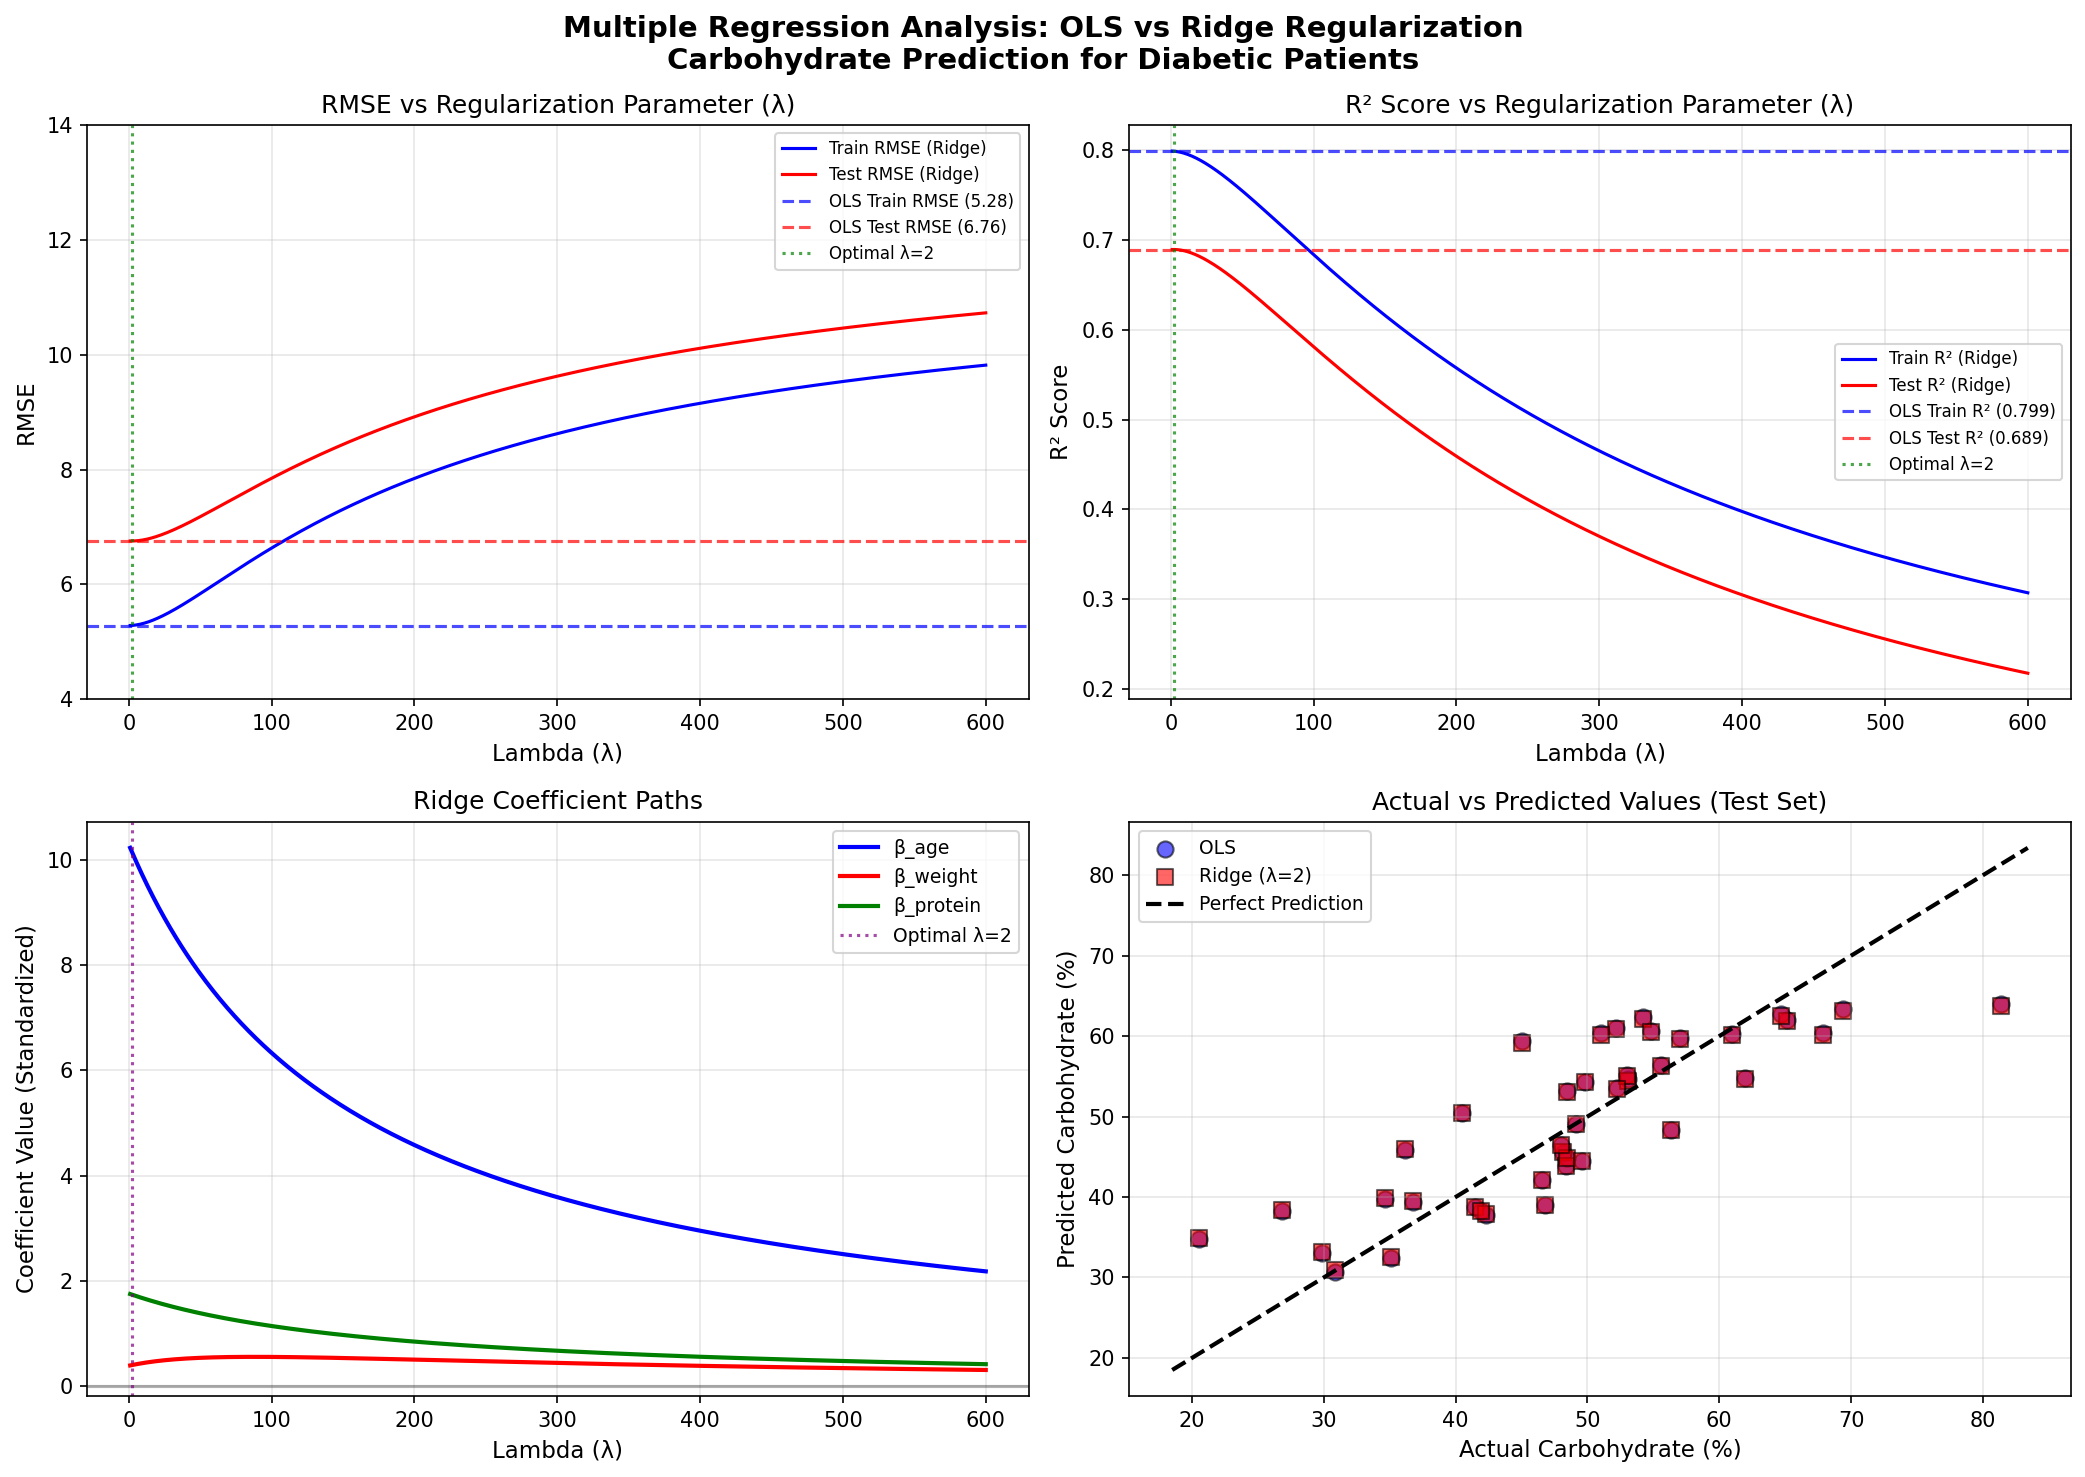
\includegraphics[width=\textwidth]{regression_analysis_plots.png}
    \caption{Multiple Regression Analysis: (a) RMSE vs $\lambda$, (b) $R^2$ vs $\lambda$, (c) Coefficient paths, (d) Actual vs Predicted values}
    \label{fig:main_plots}
\end{figure}

\begin{figure}[h]
    \centering
    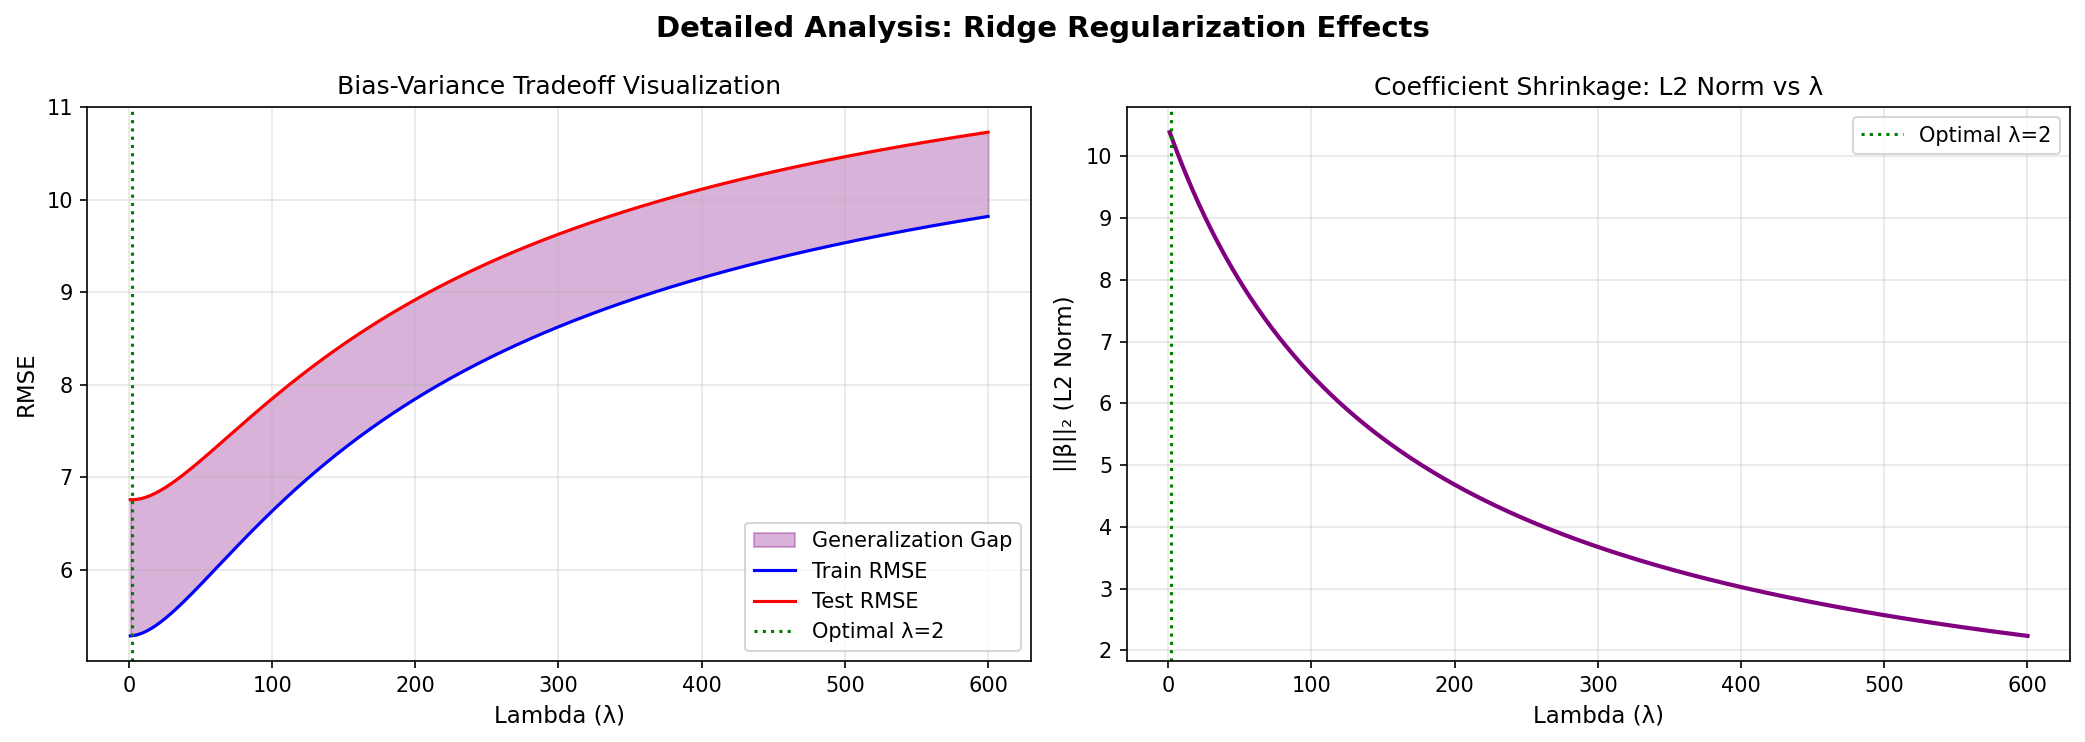
\includegraphics[width=\textwidth]{ridge_detailed_analysis.png}
    \caption{Detailed Ridge Analysis: (a) Bias-Variance Tradeoff, (b) Coefficient Shrinkage (L2 Norm vs $\lambda$)}
    \label{fig:detailed_plots}
\end{figure}

\section{Analysis and Insights}

\subsection{Coefficient Interpretation}

\textbf{Age ($\beta_{age} \approx 1.02$):} Age is the strongest predictor of carbohydrate intake. Older diabetics tend to obtain a higher percentage of their calories from complex carbohydrates. This could reflect better dietary compliance or different nutritional habits among older patients.

\textbf{Protein ($\beta_{protein} \approx 0.43$):} Protein intake has a moderate positive relationship with carbohydrate percentage. This suggests that patients who consume more protein also tend to consume more carbohydrates, possibly indicating overall higher diet compliance.

\textbf{Weight ($\beta_{weight} \approx 0.01$):} Relative body weight has a minimal effect on carbohydrate intake. This suggests that body weight is not a strong predictor of dietary compliance in this population.

\subsection{Effect of Regularization}

As the regularization parameter $\lambda$ increases:

\begin{enumerate}
    \item \textbf{Coefficient Shrinkage}: All coefficients shrink toward zero monotonically. The L2 norm $\|\boldsymbol{\beta}\|_2$ decreases from 10.39 (at $\lambda=1$) to 2.24 (at $\lambda=600$).
    
    \item \textbf{Bias-Variance Tradeoff}: Training RMSE increases (more bias), while the generalization gap (Test RMSE - Train RMSE) remains relatively stable. This indicates that regularization adds bias without significant variance reduction for this dataset.
    
    \item \textbf{Performance Degradation}: For $\lambda > 10$, both training and test performance deteriorate substantially, indicating over-regularization.
\end{enumerate}

\subsection{Why OLS Outperforms Ridge}

For this particular dataset, OLS provides better or equivalent performance compared to Ridge regression because:

\begin{itemize}
    \item The model is not overfitting (the generalization gap is reasonable)
    \item The number of samples (200) far exceeds the number of features (3)
    \item There is no severe multicollinearity among the predictors
    \item The signal-to-noise ratio is favorable for unregularized estimation
\end{itemize}

Ridge regularization is most beneficial when:
\begin{itemize}
    \item Features are highly correlated (multicollinearity)
    \item The number of features approaches or exceeds the sample size
    \item The model shows signs of overfitting (high variance)
\end{itemize}

\section{Conclusions}

\begin{enumerate}
    \item \textbf{Best Model}: OLS regression provides the best performance for this dataset, with a test RMSE of 6.76 and $R^2$ of 0.689. Ridge regression with small $\lambda$ values (1-2) provides nearly identical results.
    
    \item \textbf{Key Predictors}: Age is the dominant predictor of carbohydrate intake, followed by protein consumption. Body weight has minimal predictive power.
    
    \item \textbf{Model Fit}: The model explains approximately 69\% of the variance in carbohydrate intake, indicating a reasonably good fit for prediction purposes.
    
    \item \textbf{Regularization Effect}: While Ridge regularization successfully shrinks coefficients, it does not improve generalization for this dataset. The optimal $\lambda$ is very small (2), suggesting minimal regularization is needed.
    
    \item \textbf{Clinical Implications}: The positive relationship between age and carbohydrate intake suggests that older diabetic patients may have better compliance with high-carbohydrate dietary recommendations, which is valuable information for clinical dietary interventions.
\end{enumerate}

\section{Recommendations}

\begin{itemize}
    \item For predictive purposes on similar datasets, OLS regression is recommended due to its simplicity and equivalent performance.
    \item Cross-validation should be used for more robust $\lambda$ selection in future analyses.
    \item Consider exploring other regularization methods (Lasso, Elastic Net) if feature selection is desired.
    \item Additional features such as duration of diabetes, medication type, or socioeconomic factors could potentially improve model performance.
\end{itemize}

\clearpage
\section*{Appendix: Python Code}

\begin{lstlisting}[caption={Multiple Regression Analysis Script (Key Components)}]
import numpy as np
import pandas as pd
from sklearn.model_selection import train_test_split
from sklearn.preprocessing import StandardScaler
from sklearn.metrics import mean_squared_error, r2_score, mean_absolute_error

# Load data
data = pd.read_csv('Cabohydrate_Data.csv')
X = data[['age', 'weight', 'protein']].values
y = data['carbohydrate'].values

# Train-test split
X_train, X_test, y_train, y_test = train_test_split(
    X, y, test_size=0.2, random_state=42)

# Standardize features for Ridge
scaler = StandardScaler()
X_train_scaled = scaler.fit_transform(X_train)
X_test_scaled = scaler.transform(X_test)
y_mean = y_train.mean()
y_train_centered = y_train - y_mean

# OLS Regression (with intercept)
def ols_regression_with_intercept(X, y):
    n = len(y)
    X_aug = np.column_stack([np.ones(n), X])
    XtX = X_aug.T @ X_aug
    Xty = X_aug.T @ y
    beta = np.linalg.solve(XtX, Xty)
    return beta[0], beta[1:]  # intercept, coefficients

intercept_ols, beta_ols = ols_regression_with_intercept(X_train, y_train)

# Ridge Regression
def ridge_regression_centered(X, y, lambda_param):
    n_features = X.shape[1]
    XtX = X.T @ X
    Xty = X.T @ y
    ridge_matrix = XtX + lambda_param * np.eye(n_features)
    beta = np.linalg.solve(ridge_matrix, Xty)
    return beta

# Test lambda values from 1 to 600
lambda_values = np.arange(1, 601)
results = []

for lam in lambda_values:
    beta_ridge = ridge_regression_centered(
        X_train_scaled, y_train_centered, lam)
    y_train_pred = X_train_scaled @ beta_ridge + y_mean
    y_test_pred = X_test_scaled @ beta_ridge + y_mean
    
    rmse_train = np.sqrt(mean_squared_error(y_train, y_train_pred))
    rmse_test = np.sqrt(mean_squared_error(y_test, y_test_pred))
    r2_test = r2_score(y_test, y_test_pred)
    
    results.append({
        'lambda': lam,
        'rmse_train': rmse_train,
        'rmse_test': rmse_test,
        'r2_test': r2_test
    })

# Find optimal lambda
results_df = pd.DataFrame(results)
optimal_idx = results_df['rmse_test'].idxmin()
optimal_lambda = results_df.loc[optimal_idx, 'lambda']
print(f"Optimal lambda: {optimal_lambda}")
\end{lstlisting}

\end{document}
